% -*-LaTeX-*- 
% derived from file acl08.tex
%

\documentclass[11pt]{article}
\usepackage{acl08}
\usepackage{times}
\usepackage{latexsym}
\usepackage{amsmath}
\usepackage{dcolumn}
\usepackage{url}
\usepackage{comment}
\usepackage{graphicx}
\usepackage{qtree}
\setlength\titlebox{4.0cm}    % Expanding the titlebox

\newcommand{\blindthis}[1]{#1}
%\newcommand{\blindthis}[1]{}

\newcolumntype{d}{D{.}{.}{3}}
\DeclareMathOperator*{\corr}{corr}

\title{Automatic Syntactic MT Evaluation with Expected Dependency
  Pair Match}
% \protect\blindthis{\Thanks{Thanks to Kevin Knight for providing data for
%     earlier revisions of this research.}}

\author{\blindthis{
    Jeremy G. Kahn \and Mari Ostendorf \\
    % Signal, Speech, \& Language Interpretation Lab \\
    Signal, Speech \& Lang.\ Interpretation Lab\\
    University of Washington,
    Seattle, WA\\
    {\tt \{jgk,mo\}@ssli.ee.washington.edu}
    \And
    Brian Roark\\
    % Center for Spoken Language Understanding\\
    Ctr.\ for Spoken Lang.\ Understanding \\
    OHSU, Portland, OR\\
    {\tt roark@cslu.ogi.edu}
  }
}
\date{}


\newcommand{\headlabel}[2]{\ensuremath{\underset{\textrm{#2}}{\textrm{#1}}}}
\newcommand{\arclabel}[1]{\ensuremath{\stackrel{#1}{\to}}}
\newcommand{\DPM}[1]{\ensuremath{\mathrm{DPM}_{#1}}}
\newcommand{\DPMempty}{\ensuremath{\DPM{}}}
% \newcommand{\EDPM}[2]{
%   \DPM{ E^{#2} \left[ #1 \right] }
% }
\newcommand{\EDPM}[2]{\ensuremath{\DPM{#1}{#2}}}
\newcommand{\mDPM}[2]{\ensuremath{\DPM{#1}{0}}}
\newcommand{\bDPM}[1]{\ensuremath{\mathrm{b}\DPM{#1}}}
\newcommand{\myEDPM}[0]{\ensuremath{\mathrm{EDPM}}}
\newcommand{\BoNG}[1]{\ensuremath{\textrm{bag-of-ngrams}(#1)}}
% \newcommand{\BoNG}[1]{
%   \ensuremath{F_\cup \left(n_1^{#1}  \textrm{-gram} \right)
%   }}
\newcommand{\bBoNG}[1]{\ensuremath{\textrm{av-bags-of-ngrams}(#1)}}
% \newcommand{\bBoNG}[1]{
%   \ensuremath{F_\forall \left(
%       n_1^#1\textrm{-gram}
%     \right)}}

\newcommand{\ngram}[0]{\ensuremath{n\textrm{-gram}}}
\newcommand{\precision}[0]{\ensuremath{\textrm{Precision}}}
\newcommand{\recall}[0]{\ensuremath{\textrm{Recall}}}

\begin{document}
\maketitle
\begin{comment}
  \begin{abstract}
    Previous work on dependency-based machine translation evaluation
    has shown that an LFG-based F-measure of labeled partial
    dependencies over an $n$-best list has improved correlation with
    human judgments of fluency and adequacy as compared to BLEU and
    TER.  Inspired by \textsc{SParseval}, we create Expected
    Dependency Pair Match and show that a statistical syntactic parser
    may be used in place of LFG dependencies. We explore variations on
    other aspects of the dependency-matching method, including a
    principled weighting of the $n$-best trees and using simple words
    (along with partial dependencies).
  %
    % We find that including $n>1$ parses helps, especially if one
    % incorporates probabilistic weights from the parser.
    % Additionally, we find that matching simple words (along with
    % partial-dependencies) further improves correlations with human
    % judgments.

    Our experiments suggest that $\Delta$\myEDPM{} is superior to
    $\Delta$BLEU and $\Delta$TER as a per-document and per-sentence
    predictor of $\Delta$HTER.

    % From these results, we design a new scoring metric ``Expected
    % Dependency Pair Match'' (\myEDPM), and demonstrate that
    % $\Delta$\myEDPM{} is superior to $\Delta$BLEU and $\Delta$TER as
    % a per-document and per-sentence predictor of $\Delta$HTER.
  \end{abstract}
\end{comment}
% \section*{Introduction}
% This paper presents the Expected Dependency Pair Match metric and
% algorithm.  This algorithm uses a popular PCFG parser to extract
% expected counts of dependency structures from hypothesis and reference
% translations and score them.

% The remainder of this work describes the motivation for this
% algorithm, and presents a series of experiments exploring its
% correlation with human judgments and its correlation with the
% human-targeted HTER metric.

% \section{Background \& Motivation}

In improving MT metrics, we try to model acceptable variation, whether
by modeling word-choice (e.g.\ METEOR \cite{banerjee05meteor}), by weighting adjacent
matches more than non-local matches (e.g.\ GTM \cite{turian03mteval})
or by modeling syntactic information \cite{liu05syntaxformteval}.
\newcite{owczarzak07labelleddepseval} explore the correlation of their
dependency-syntax based measure \textbf{d} and \textbf{d\_var} with
human judgment, and report substantial improvements relative to the
popular measures BLEU and TER.

In keeping to the syntactic approach, we present Expected Dependency
Pair Match (\myEDPM{}), which follows and extends
the labelled-dependency match version of \textsc{SParseval}
\cite{roark06:sparseval} and the \textbf{d}/\textbf{d\_var}
\cite{owczarzak07labelleddepseval} measures. These approaches evaluate
hypothesis-reference similarity with an $F$ measure over fragments of
a labelled dependency structure, which may be generated by a PCFG with
deterministic head-finding
\cite{liu05syntaxformteval,roark06:sparseval} or by extracting the
semantic dependencies from an LFG parser (\newcite{cahill04lfg} in
\newcite{owczarzak07labelleddepseval}).  

\myEDPM{} extends these partial-dependency-scoring strategies with a widely
used and publically available PCFG parser and deterministic
head-finding rules instead of an LFG system. In addition, it
incorporates word-level matching and weighted multiple parse
alternatives for improved performance.


\section{Definition of \DPMempty{} family of metrics}
\label{sec:dpm}
We define a family of Dependency Pair Match (\DPMempty{}) measures
that is composed of extensions of the methods described inr
\newcite{owczarzak07labelleddepseval}.  \DPMempty{} is defined as the
$F$ measure over bags-of-subtrees of the hypothesis translation
dependency tree as compared to bags-of-subtrees of the reference
translation dependency tree.
%
\begin{figure*}
  \centering
  \begin{tabular}{rcc}
    & \textbf{Reference} & \textbf{Hypothesis} \\
    \textbf{dependency tree}
    & 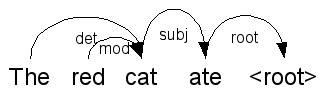
\includegraphics[scale=0.5]{dpm-example-ref.png} & 
    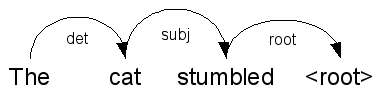
\includegraphics[scale=0.5]{dpm-example-hyp.png}\\
    \textbf{$dlh$ list} &
    {\small \begin{tabular}{@{$\langle$}c@{,~}c@{,~}c@{$\rangle$}}
      the & \arclabel{\texttt{det}}  &  cat \\
      red & \arclabel{\texttt{mod}}  &  cat \\
      cat & \arclabel{\texttt{subj}} &  ate \\
      ate & \arclabel{\texttt{root}} &  $<$root$>$ \\
    \end{tabular}} & 
    {\small \begin{tabular}{@{$\langle$}c@{,~}c@{,~}c@{$\rangle$}}
      the &      \arclabel{\texttt{det}}  &  cat \\
      cat &      \arclabel{\texttt{subj}} &  stumbled \\
      stumbled & \arclabel{\texttt{root}} &  $<$root$>$ \\
    \end{tabular}} \\
  \end{tabular}\\
  Precision$_{dlh}$ is $\frac{1}{3}$ and Recall$_{dlh}$ is
  $\frac{1}{4}$, yielding  $\DPM{dlh} = F = \frac{2}{7} = 0.286$
  \caption{Example hypothesis and reference dependency trees and the $dlh$ decomposition of each.}
  \label{fig:dpmexample}
\end{figure*}
Figure~\ref{fig:dpmexample} demonstrates a toy example of the
bags-of-dependencies extracted from a hypothesis and reference
tree.  In the example presented here, we extract only $dlh$
dependencies, which are tuples of the form $\langle \textrm{Dependent},
\textrm{arc-Label}, \textrm{Head} \rangle$.
% JGK: factor part of this back in?
% We describe different variants in this family below, and compare their
% effectiveness in section~\ref{sec:facorr}.

\subsection{\DPMempty{} variations in subtree extraction}
Different members of the \DPMempty{} family of metrics may extract
different subtrees.  We denote the set of extracted tree-components
with a trailing subscript: \DPM{dlh} extracts all $\langle
\textrm{Dependent}, \textrm{arc-Label}, \textrm{Head} \rangle$ subtree
tuples, roughly equivalent to labeled \textsc{SParseval}
\cite{roark06:sparseval} and the \newcite{owczarzak07labelleddepseval}
\textbf{d} measure. We also consider the $\DPM{1g,2g}$ extractions,
which represent unigrams and bigrams, or the \DPM{dl,lh}, which
extracts all the subtrees $\langle \textrm{Dependent},
\textrm{arc-Label} \rangle$ and $\langle \textrm{arc-Label},
\textrm{Head} \rangle$ (roughly equivalent to the
\newcite{owczarzak07labelleddepseval} \textbf{d\_var} method).

\subsection{\DPMempty{} variations using $n$-best lists and expected counts}
%% Multiple parses
Since the dependency structures of the hypothesis and reference text
are hidden, we also  explore alternative
dependency structures predicted by the parser, to cope with genuine
ambiguity (in both hypothesis and reference) and to
mitigate the effects of parser error. \DPMempty{} is well-defined over
the $n$-best list of dependency-structures: when $n>1$, \DPMempty{}
uses the expectation of bags-of-subtrees rather than the
bags-of-subtrees derived from the 1-best parse.

An expectation requires a probability distribution over the $n$-best
list, and we ``flatten'' the parser probabilities such that
$\tilde{p}(x) = \frac{p(x)^\gamma}{\sum_ip(i)^\gamma}$ (where $\gamma$
is a free parameter) to account for over-confidence in the parser.  In
all cases, the probabilities are normalized to sum to one over the the
$n$-best list.

\subsection{Implementation of the \DPMempty{} family}
\label{sec:implementation}
In principle, the \DPM{} family of measures may be implemented with
any parser that generates a dependency graph (a single labelled arc
for each word, pointing to its head-word). 

% JGK: tighten this up
Our reference implementation\footnote{Download the EDPM source code
  --- a collection of Perl scripts and libraries --- at
  \url{http://ssli.ee.washington.edu/people/jgk/dist/edpm/}, or contact
  the first author.}
uses a state-of-the-art PCFG parser (the first stage
of \newcite{charniak-johnson:2005:ACL}) to generate a 50-best list of
trees for each hypothesis and reference translation, using the
parser's default WSJ % Wall Street Journal 
training parameters.
%
We use \newcite{magerman95headfinding} head-finding to construct
dependency trees, using the Charniak parser's head-finding rules, with
three modifications: prepositional and complementizer phrases choose
nominal and verbal heads respectively and auxiliary verbs are
modifiers of main verbs (rather than the converse).

Arc-labels $d
\stackrel{A/B}{\to} h$ are determined from constituent labels, where the arc
label $A/B$ between dependent $d$ and its head $h$ is composed of $A$
(the lowest constituent headed by $h$ and dominating $d$) and
$B$ (the highest constituent headed by $d$).
%
This strategy is the one adopted in labelled-dependency
\textsc{SParseval}, and it acts as an approximation of the rich
semantics generated by \cite{cahill04lfg} or another heavily
knowledge-engineered parser, but with much less knowledge-engineering
required.
%
The $A/B$ labels are not as descriptive as the LFG semantics, but they
have a similar resolution, e.g.\ the $\stackrel{S/NP}{\to}$ arc label
usually represents a subject dependent of a sentential verb.

\subsection{Optimal EDPM}
Experiments exploring correlation with fluency and adequacy judgments
against the LDC Multiple Translation Chinese corpus parts
2~\cite{LDC03MTC2} and 4~\cite{LDC06MTC4} indicate that the best
member of the \DPMempty{} family uses the full 50-best parses
produced by the system, with a ``flattening'' $\lambda=0.25$.  Using
both the partial subtrees $dl,lh$ and the string-only statistics
$1g,2g$ provides an optimal setting of
\begin{displaymath}
  \myEDPM{} = \DPM{1g,2g,dl,lh}, n=50, \gamma=0.25
\end{displaymath}
This configuration for \myEDPM{} has a correlation $r=0.240$ against the
average fluency and adequacy judgment per-sentence over these corpora.


\section{Correlations with HTER}
\label{sec:hter}

We explore this \myEDPM{} variant's utility on another task:
predicting the human-targeted translation edit rate (HTER) on the
(unsequestered) GALE 2.5 evaluation results, and find that
per-document differences across systems in \myEDPM{} ($\Delta$\myEDPM)
are better correlated with changes in HTER ($\Delta$HTER) than
$\Delta$BLEU$_4$ or $\Delta$TER (table~\ref{tab:hter:perdoc1}).

\begin{table}
  \centering
  \begin{tabular}{r|r|r||r}
     \multicolumn{1}{c|}{Measure $s$} 
     & \multicolumn{1}{c|}{all-Arabic} &
     \multicolumn{1}{c||}{all-Chinese} &\multicolumn{1}{c}{all}\\
    \hline{}
    TER      &  0.51 &  0.19 &  0.39 \\
    BLEU$_4$ & -0.40 & -0.19 & -0.32 \\
    \myEDPM  & 
       \textbf{-0.61}&
               \textbf{-0.25}&
                       \textbf{-0.47}\\
  \end{tabular}
  \caption{Per-document Pearson's $r$ of $\Delta s$ with $\Delta\textsc{hter}$ over
    various measures $s$, examined for each genre in the corpus, for each
    language in the corpus, and as a whole. }
  \label{tab:hter:perdoc1}
\end{table}
\begin{comment}
  We compare \myEDPM{}'s correlation with HTER against both that of
  TER and that of BLEU$_4$, two very popular automatic measures.
\end{comment}
It is worth mentioning that TER has an advantage in that HTER uses a
TER measure to calculate the post-editing work between the
hypothesized translation and the human-targeted reference which could,
in principle, bias HTER towards a TER measure. \myEDPM{} shares no
such advantage.  \myEDPM{} nevertheless has the best correlation of
the three measures in both Arabic and Chinese, as well as over the
entire corpus.
\section{Conclusion and future work}
\label{sec:conclusion}

\myEDPM{} demonstrates a promising direction in exploiting syntactic
structure for automatic evaluation of machine translation hypotheses.
It differs in nature from other proposed evaluation methods in that it
does \emph{not} use word-substitution tables or tuned weights (beyond
the $\lambda$ free parameter described above), and yet substantially
outperforms BLEU$_4$ and TER as a predictor of changes to HTER.

In future work, we would like to explore a number of related
questions.  Exploring a larger list of parse possibilities (by
increasing $n$ or scoring from packed parse forests
\cite{huang08parseforests}) might allow better diversity of link types
and better estimates of their expected counts.  Alternatively, we may
use a different PCFG parser as another way of exploring the trade-offs
between parse-quality, MT quality prediction, and speed.  On the other
hand, a poor-quality translation that is very difficult to parse may
interfere with the quality of the measure; assessing this measure's
sensitivity to sentence quality would also be worthwhile. In a
different direction, we would like to ask whether other segmentations
of the dependency tree are more appropriate than those explored here,
following up on an approach suggested in
\newcite{liu05syntaxformteval}, which uses linked words in chains much
larger than 2.

From the results correlating \myEDPM{} with both HTER and human
judgments of fluency and accuracy, \myEDPM{} seems to be a superior
tool for identifying improvements at the document level and at the
sentence level, which is often where parameter tuning takes place. One
possible use for this measure, since it is more computationally-costly
than BLEU or TER, might be as a late pass evaluation metric in
training to select among translation outputs already deemed to be very
good.

\section*{Acknowledgments}

{\small
\blindthis{This material is based upon work supported by the National
  Science Foundation under Grant No.\ 0741585 and the Defense Advanced
  Research Projects Agency under Contract No.\ HR0011-06-C-0023.

  Any opinions, findings, and conclusions or recommendations expressed
  in this material are those of the author(s) and do not necessarily
  reflect the views of the National Science Foundation or the Defense
  Advanced Research Projects Agency.}
}


% MO: TO DO Could save space by using first initials.
\bibliographystyle{acl}
\bibliography{edpm-summary}

\end{document}
